Proper evaluation methods guide researchers in choosing the model that best fits their needs. This chapter is dedicated to the most common evaluation metrics adopted by academics in the field of electricity forecasting. Error metrics and measures vary depending on whether we are concerned with point or probabilistic forecasts. Additionally, note that the latter can take different forms which therefore requires different measures.
\section{Mean absolute error}\label{mae}
Consider the time series with actual values given by $y=(y_{n+1}, y_{n+2},\dots, y_{n+h})$
and its $h$ step ahead point forecast $\hat{y}=(\hat{y}_{n+1}, \hat{y}_{n+2},\dots, \hat{y}_{n+h})$ the mean absolute error (MAE) is defined as
\begin{definition}
    The mean absolute error is defined as
    $$
    \mathrm{MAE}(y,\hat{y})=\frac{1}{h}\| y- \hat{y}\|_{1}=\frac{1}{h}\sum\limits_{k=1}^{h}|y_{n+k}-\hat{y}_{n+k}|
    $$
\end{definition}

\section{Root mean squared error}\label{rmse}
\begin{definition}
    The root mean squared error is defined as
    $$
    \mathrm{RMSE}(y, \hat{y})=\frac{1}{\sqrt{h}}\|y-\hat{y}\|_{2}=\sqrt{\frac{\sum\limits_{k=1}^{h}(y_{n+k}- \hat{y}_{n+k})^2}{h}}
    $$
\end{definition}

Mean absolute error and root mean squared error posses the useful property of being expressed in the same units of the data, thus enabling meaningful comparisons.
However, a drawback of such measures is that we cannot use them to compare accuracy between time series which have different magnitudes. For instance, a day ahead error of 1kWh is negligible when considering a daily demand of 100kWh while the same error is considerably big when daily demand is 2kWh. This consideration leads to relative accuracy scores. Between those the mean absolute percentage error (MAPE) is by far the most popular.


\section{Mean absolute percentage error}\label{mape}. 
\begin{definition}
    The mean absolute percentage error is defined as
    $$
    \mathrm{MAPE}(y,\hat{y})=\frac{100}{h}\sum\limits_{k=1}^{h}\frac{|y_{n+k}-\hat{y}_{n+k}|}{|y_{n+k}|}$$
\end{definition}

\section{Root mean squared percentage error}\label{rmspe}
\begin{definition}
    The root mean squared percentage error is defined as
    $$
    \mathrm{RMSPE}(y,\hat{y})=100\cdot\sqrt{\frac{1}{h}\sum\limits_{k=1}^{h} \left(\frac{|y_{n+k}-\hat{y}_{n+k}|}{|y_{n+k}|}\right)^2}
    $$
\end{definition}
Mean absolute percentage error and root mean squared percentage error may not be appropriate for series which have zero or very small values, for example, electricity demand at the household level. The result is a large score regardless of the absolute errors.
Scaled errors constitute a robust family of scores.
\section{Mean absolute scaled error}\label{mase}
\begin{definition}
    The mean absolute scaled error is defined as
    $$
    \mathrm{MASE}(y,\hat{y})=\frac{1}{h}\sum\limits_{k=1}^h\frac{|y_{n+k}-\hat{y}_{n+k}|}{\frac{1}{h-1}\sum\limits_{k=2}^{h}|y_{k}-y_{k-1}|}
    $$
\end{definition}
In the denominator we have the error of the naïve/persistence model. 
In this model, the current demand makes up the prediction for the next time step, that is $\hat{y}^{\mathrm{naive}}_{n+1}=y_{n}$.
\section{Root mean squared scaled error}\label{rmsse}
\begin{definition}
    The root mean squared scaled error is defined as
    $$
    \mathrm{RMSSE}(y,\hat{y})=\sqrt{\frac{1}{h}\sum\limits_{k=1}^h\left(\frac{|y_{n+k}-\hat{y}_{n+k}|}{\frac{1}{h-1}\sum\limits_{k=2}^{h}|y_{k}-y_{k-1}|}\right)^2}
    $$
\end{definition}


\section{Pinball score}\label{pinball}
The pinball score or quantile score is used to measure the accuracy of a quantile forecast.
\begin{definition}
    The pinball loss is defined as
    $$
    \mathrm{Pinball}(y_{t},\hat{y}_{t,q},q)=
\begin{cases}
(q-1)(\hat{y}_{t,q}-y_{t}) & y_t > \hat{y}_{t,q} \\
q(\hat{y}_{t,q}-y_t) & y_t \leq \hat{y}_{t,q}
\end{cases}
$$
\end{definition}
The pinball loss is an asymmetric function, it weights its score differently depending on the error sign and on the quantile considered, see Figure \ref{fig:pinball}.
\begin{figure}
    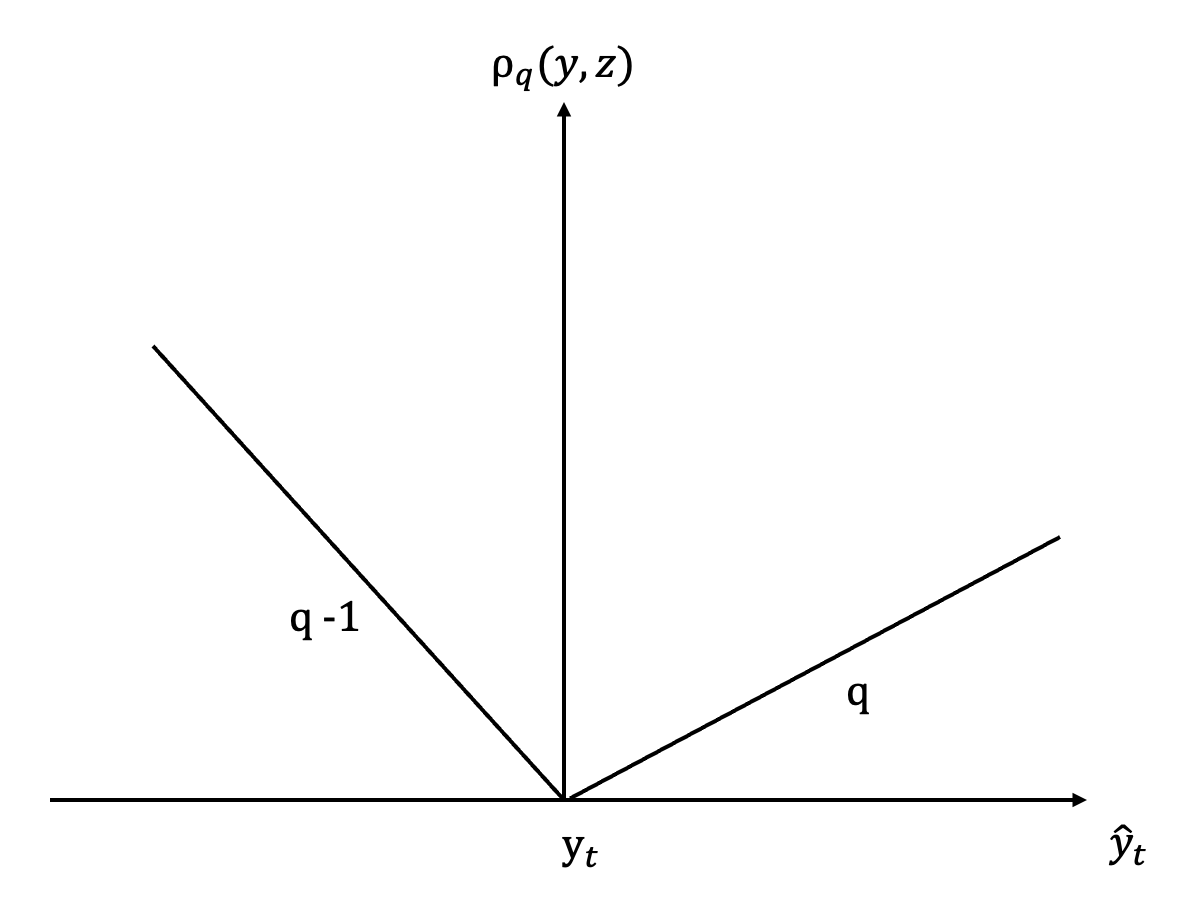
\includegraphics[width=\textwidth]{images/pinball_loss.png}
    \caption{Pinball loss}
    \label{fig:pinball}
  \end{figure}
By averaging all the pinball losses over all quantiles and over the whole forecast horizon, we obtain the pinball loss of the probabilistic forecast.
\section{Winkler score}
\begin{definition}
    The Winkler score is defined as
    $$
    \mathrm{Winkler}(y_t,  u_{t},l_{t},\alpha)=\begin{cases}
        \delta & l_{t}\leq y_{t}\leq u_{t}\\
        \delta+2(l_{t}-y_{t})/\alpha & y_{t}< l_{t}\\
        \delta+2(l_{t}-u_{t})/\alpha & y_{t} \geq u_{t}
    \end{cases}
    $$
\end{definition}
Where $\delta$ is the prediction interval (PI) width, that is $\delta=u_t-l_t$, $\alpha$ is (1-coverage level), $u_t$ is the prediction interval upper threshold and $l_t$ is the prediction interval lower threshold at time step $t$. This score penalises observations falling outside the prediction interval and rewards narrow prediction intervals.
\section{Continous ranked probability score}
The continous ranked probability score (CRPS) measures the difference between the estimated cumulative distribution $\hat{F}$ and the empirical cumulative density function (CDF).
\begin{definition}\label{def_crps}
    The continous ranked probability score is defined as
    $$
    \mathrm{CRPS}(y, \hat{F})=\int\limits_{-\infty}^{\infty}\left(\hat{F}(x)-\mathbb{I}_{\{x-y\}} \right)^2 dx
    $$
\end{definition}
% Nevertheless, we can evaluate the integral in closed form. 
Where the indicator function is defined as 
    $$\mathbb{I}_{\{z\}}=
\begin{cases}
0, & z<0\\
1, & z \geq 0
\end{cases}$$
\\
For a visualisation see Figure \ref{fig:crps}. The grey area is what contributes toward the CRPS score.
The better the estimated cumulative density function is the smaller the total CRPS score will be.
\begin{figure}
    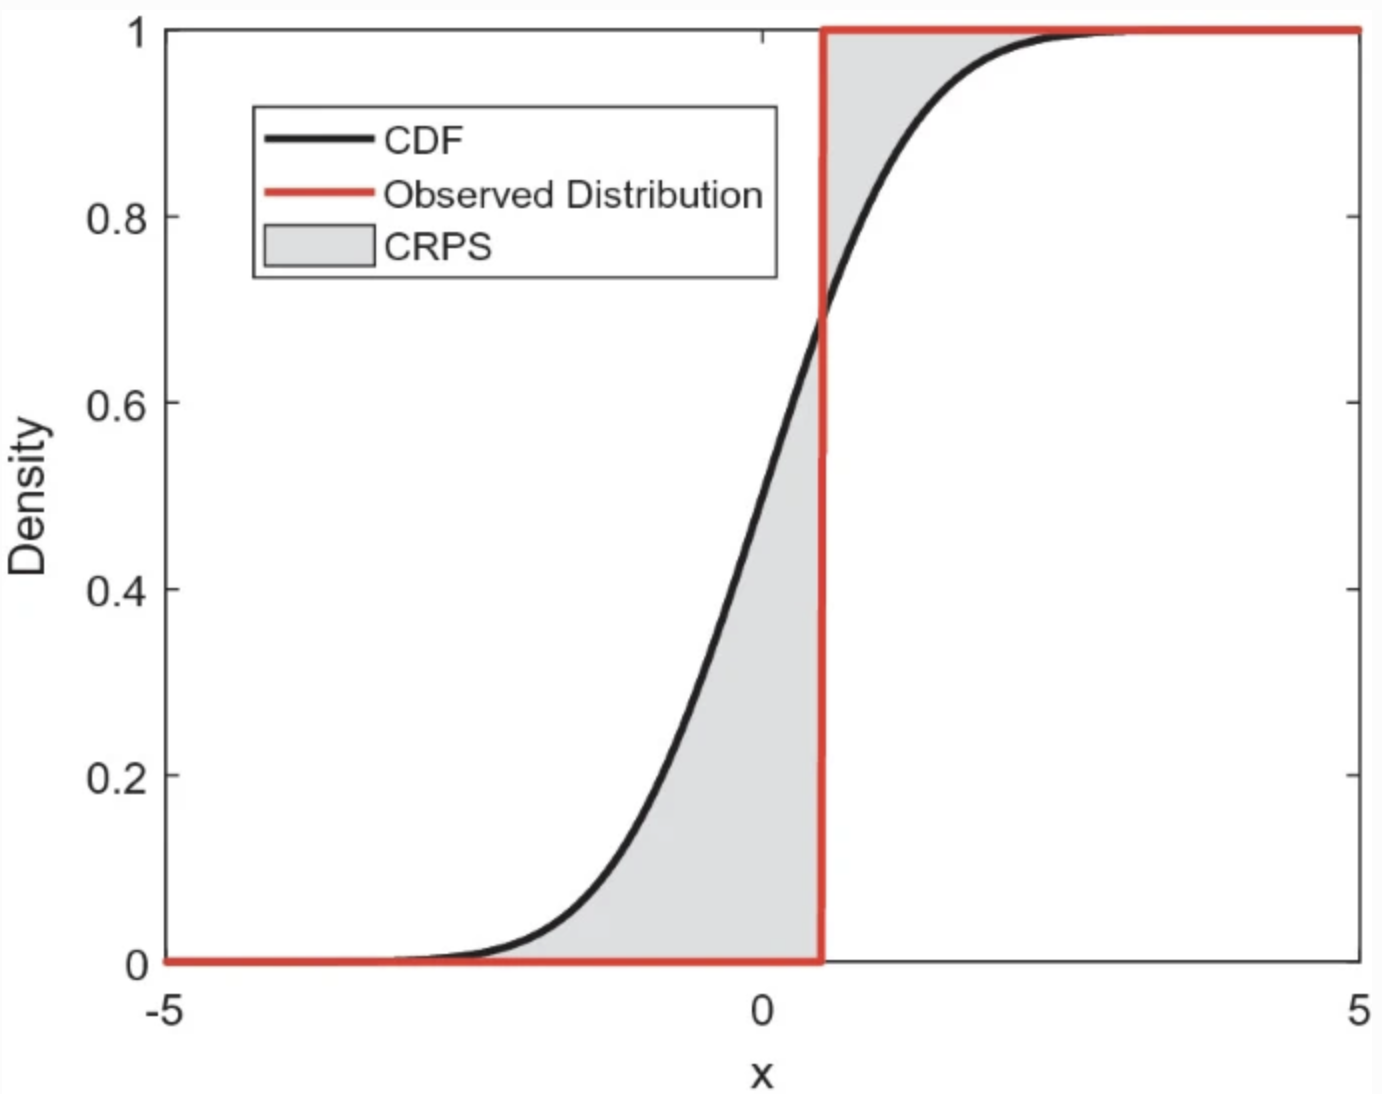
\includegraphics[width=\textwidth]{images/crps.png}
    \caption{CRPS integral \cite{haben2023core}}
    \label{fig:crps}
  \end{figure}
It is worth noting, that the CRPS integral can be rewritten in terms of expectations. This makes its evaluation easier, since we know that the sample mean converges to the expectation for sufficiently big sample sizes by the law of large numbers. This was first pointed out by \cite{proper_scores}, where the authors take advantage of Lemma 2.2 of \cite{new_multi_test2} or equivalently identity (17) of \cite{new_multi_tes1}.
\\
\begin{lemma}
    Let $X_1$, $X_2$, $Y_1$, $Y_2$ be independent real random variables with finite expectations. Let $X_1,X_2$ be identically distributed with distribution function $F$ and let $Y_1,Y_2$ be identically distributed with distribution function $G$. Then
   \begin{equation}\label{eq:crps_expectation}
    \mathbb{E}(|X_1-Y_1|)-\frac{1}{2}\mathbb{E}(|X_1-X_2|)-\frac{1}{2}\mathbb{E}(|Y_1-Y_2|)=\int\limits_{-\infty}^{\infty}\left(F(x)-G(x)\right)^2dx
\end{equation}
\end{lemma}
Notice that, in our case, Equation \ref{eq:crps_expectation}, the distribution $G$ of $Y_1$ and $Y_2$ is degenerate, with all probability mass on a single point $y$.
%  (x notation will need to be cleaned here). Since $G(t)=:$
It follows that the third addend in the summation is zero. That is because $Y_1$ and $Y_2$ both following distribution $G$ implies that $\mathbb{E}(|Y_1-Y_2|)$ corresponds to the difference of two equal constant numbers.

Additionally, since $Y_1$ is just a constant, we have $Y_1=y$.

Putting everything together we have obtained an alternative way of computing the CRPS score.
\begin{equation}
    \int\limits_{-\infty}^{\infty}\left(\hat{F}(x)-\mathbb{I}_{\{x-y\}} \right)^2 dx=\mathbb{E}(|X_1-y|)-\frac{1}{2}\mathbb{E}(|X_1-X_2|)
\end{equation}

\section{Probability integral transform}
The probability integral transform (PIT) is a method to assess visually the quality of a probabilistic forecast. PIT is obtained by applying the predicted cumulative density function $\hat{F}$ to the data. If applying such CDF to the data results in a uniform distributed PIT, then $\hat{F}$ is a valid prediction. If not, $\hat{F}$ is not a good estimate of the CDF for the considered data. Figure \ref{fig:pit} provides an example, applying the true CDF results in a well calibrated PIT (left). Alternatively, applying a bad CDF results in either an overdispersed (middle) or underdispersed (right) PIT.
\begin{figure}
    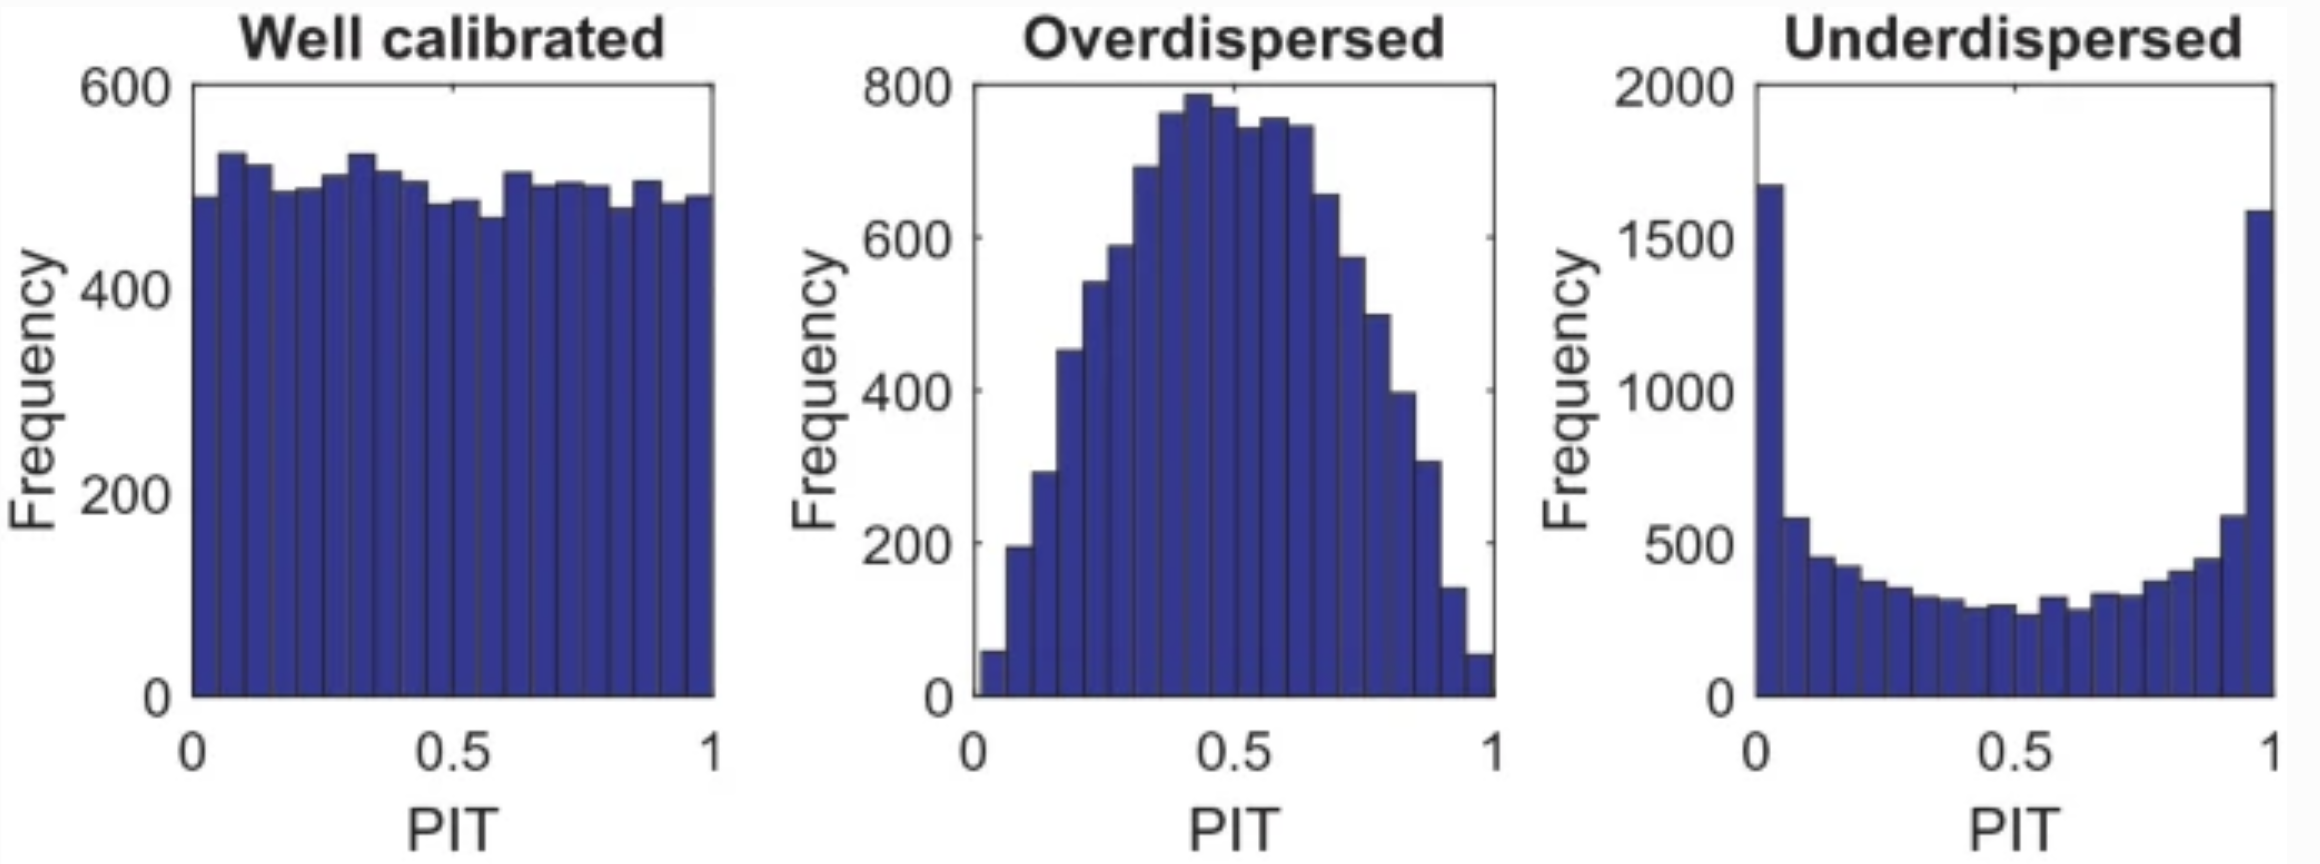
\includegraphics[width=\textwidth]{images/pit.png}
    \caption{Probability integral transform types \cite{haben2023core}}
    \label{fig:pit}
  \end{figure}

%RELIABILITY PLOT
%PICP,NMPIW,CWC,unconditional coverage(arora)-->Probability density forecasting of wind speed based on quantile regression and kernel density estimation Lei Zhang

% Reliability and sharpness \section{Criteria}-->Recent advances in electricity price forecsating a review of probabilistic forecasting Weron
% Two criteria are used in literature to evaluate probabilistic forecasting: sharpness and reliability. Reliability means 